% =====================================================================
%  Project Report: Basic Battery Management System (ESP32 + INA226)
%  Compile from the docs/ folder:  pdflatex report.tex  (run twice)
%  Screenshots are taken from ../images/ (see images/README.md)
% =====================================================================
\documentclass[12pt,a4paper,oneside]{report}

% ---------------- Edit these details ----------------
\newcommand{\studentname}{Harshil Valecha}
\newcommand{\rollno}{[Roll Number]}
\newcommand{\institute}{[Institute Name]}
\newcommand{\department}{[Department Name]}
\newcommand{\course}{Embedded Systems}
\newcommand{\semester}{Semester V}
\newcommand{\guide}{[Faculty Guide Name]}
\newcommand{\wokwiurl}{https://wokwi.com/projects/481598958521700353}
\newcommand{\githuburl}{[GitHub Repository URL]}
% ----------------------------------------------------

\usepackage[margin=2.5cm]{geometry}
\usepackage[T1]{fontenc}
\usepackage{lmodern}
\usepackage{amsmath}
\usepackage{graphicx}
\usepackage{float}
\usepackage{booktabs}
\usepackage{tabularx}
\usepackage{array}
\usepackage{enumitem}
\usepackage{xcolor}
\usepackage{listings}
\usepackage{caption}
\usepackage{fancyhdr}
\usepackage{titlesec}
\usepackage{tikz}
\usetikzlibrary{shapes.geometric, arrows.meta, positioning, calc}
\usepackage[hidelinks]{hyperref}

% ---------------- Style ----------------
\definecolor{accent}{RGB}{0,90,140}
\definecolor{codebg}{RGB}{246,248,250}
\definecolor{codecomment}{RGB}{106,115,125}
\definecolor{codekw}{RGB}{0,92,197}
\definecolor{codestr}{RGB}{3,47,98}

\titleformat{\chapter}[hang]{\Huge\bfseries\color{accent}}{\thechapter.}{0.6em}{}
\titlespacing*{\chapter}{0pt}{0pt}{20pt}
\titleformat{\section}{\Large\bfseries\color{accent}}{\thesection}{0.6em}{}
\titleformat{\subsection}{\large\bfseries}{\thesubsection}{0.6em}{}

\pagestyle{fancy}
\fancyhf{}
\fancyhead[L]{\small Basic Battery Management System}
\fancyhead[R]{\small \studentname}
\fancyfoot[C]{\thepage}
\renewcommand{\headrulewidth}{0.4pt}
\fancypagestyle{plain}{\fancyhf{}\fancyfoot[C]{\thepage}\renewcommand{\headrulewidth}{0pt}}

\setlength{\parskip}{0.5em}
\setlength{\parindent}{0pt}
\setlist{itemsep=2pt, topsep=4pt}
\renewcommand{\arraystretch}{1.3}

\lstdefinestyle{code}{
  language=C++,
  backgroundcolor=\color{codebg},
  basicstyle=\ttfamily\footnotesize,
  keywordstyle=\color{codekw}\bfseries,
  commentstyle=\color{codecomment}\itshape,
  stringstyle=\color{codestr},
  numbers=left, numberstyle=\tiny\color{gray}, numbersep=8pt,
  frame=single, rulecolor=\color{gray!40},
  breaklines=true, showstringspaces=false, tabsize=2,
  morekeywords={uint8_t,uint16_t,uint32_t,int16_t,int32_t,pin_t,timer_t,bool,true,false},
  xleftmargin=1.5em, framexleftmargin=1.5em
}
\lstset{style=code}

% Screenshot: includes ../images/<file> if present, otherwise a placeholder box
\newcommand{\screenshot}[3]{%
  \begin{figure}[H]\centering
  \IfFileExists{../images/#1}%
    {\includegraphics[width=0.92\linewidth,height=0.42\textheight,keepaspectratio]{../images/#1}}%
    {\fbox{\parbox[c][5cm][c]{0.85\linewidth}{\centering\color{gray}\itshape Screenshot to be added:\\[4pt]\texttt{images/#1}}}}%
  \caption{#2}\label{#3}
  \end{figure}}

% =====================================================================
\begin{document}

% ---------------- Title page ----------------
\begin{titlepage}
\centering
\vspace*{1cm}
{\Large \institute\par}
{\large \department\par}
\vspace{2cm}
{\large Project Report\par}
\vspace{0.4cm}
{\color{accent}\rule{\linewidth}{1.2pt}\par}
\vspace{0.4cm}
{\huge\bfseries Basic Battery Management System\\[6pt] \Large State of Charge Estimation using ESP32 and INA226\par}
\vspace{0.4cm}
{\color{accent}\rule{\linewidth}{1.2pt}\par}
\vspace{2cm}
{\large Submitted by\par}
\vspace{0.2cm}
{\Large\bfseries \studentname\par}
{\large \rollno\par}
\vspace{1.5cm}
{\large Course: \course \quad|\quad \semester\par}
\vspace{0.3cm}
{\large Under the guidance of: \guide\par}
\vfill
{\large November 2026\par}
\end{titlepage}

% ---------------- Abstract ----------------
\pagenumbering{roman}
\chapter*{Abstract}
\addcontentsline{toc}{chapter}{Abstract}

Batteries power almost every portable and remote electronic device, yet many simple devices estimate the remaining charge only from the battery voltage. This is inaccurate, because the voltage of a battery drops when a load is connected and rises again when the load is removed. Such errors lead to sudden shutdowns, over-discharge and a shorter battery life.

This project presents a basic Battery Management System (BMS) that monitors a single 3.7\,V Li-ion cell and estimates its State of Charge (SoC). The system uses an ESP32 microcontroller and an INA226 high-precision current and voltage sensor connected over the I\textsuperscript{2}C bus. At start-up, the SoC is estimated from the resting battery voltage using a Li-ion lookup table with linear interpolation. After that, the SoC is tracked every second using \emph{coulomb counting}, i.e.\ by integrating the measured current over time. The system displays voltage, current, operating mode (Charging, Discharging or Idle), SoC, remaining capacity and battery status (LOW, OK or FULL) on the Serial Monitor.

Since the physical sensor was not available, the complete system was developed and tested in the Wokwi online simulator. Wokwi has no INA226 or battery model, so two custom simulated chips were written in C: a Li-ion cell whose voltage depends on its charge, and an INA226 that responds over I\textsuperscript{2}C exactly like the real device. As a result, the same firmware runs in simulation and on real hardware. Testing showed correct detection of all operating modes, and the SoC calculated by the ESP32 changed at exactly the same rate as the actual charge of the simulated battery.

\tableofcontents
\listoffigures
\listoftables

\clearpage
\pagenumbering{arabic}

% =====================================================================
\chapter{Introduction}

\section{Background}
Rechargeable batteries, especially lithium-ion (Li-ion) cells, are used in mobile phones, laptops, electric vehicles, solar energy storage, drones, medical devices and IoT sensor nodes. In all of these, the user needs to know how much energy is left in the battery, in the same way a driver needs a fuel gauge. This quantity is called the \textbf{State of Charge (SoC)} and is expressed as a percentage of the full capacity.

A \textbf{Battery Management System (BMS)} is the electronic system that monitors a battery and keeps it in a safe and useful operating range. A complete BMS performs many tasks, such as measurement, SoC estimation, protection, cell balancing and communication. This project focuses on the most visible and most important of these: measuring the battery and estimating its SoC accurately.

\section{Problem Statement}
Many low-cost devices estimate the battery level only from the battery voltage. This method is simple but unreliable because:
\begin{itemize}
  \item the battery voltage \textbf{drops under load} due to internal resistance and recovers at rest, so the displayed level jumps up and down;
  \item the voltage curve of a Li-ion cell is \textbf{fairly flat} in the middle range, so a small voltage error causes a large SoC error;
  \item wrong SoC values cause \textbf{sudden shutdowns}, over-discharge or overcharge, which reduce battery life and can be unsafe.
\end{itemize}

\section{Objectives}
\begin{enumerate}
  \item Measure the battery voltage and current accurately using the INA226 sensor.
  \item Estimate the initial SoC from the battery's resting voltage.
  \item Track the SoC continuously using coulomb counting.
  \item Detect the operating mode: Charging, Discharging or Idle.
  \item Display voltage, current, SoC, remaining capacity and status on the Serial Monitor.
  \item Build and verify the complete system in the Wokwi simulator, using code that also runs unchanged on real hardware.
\end{enumerate}

\section{Scope}
The project covers a single 3.7\,V Li-ion cell with currents up to about 0.8\,A. Protection (cut-off switches), temperature measurement, multi-cell balancing and wireless communication are outside the current scope and are listed as future work.

\section{Organisation of the Report}
Chapter~\ref{ch:background} explains the theory behind SoC estimation. Chapter~\ref{ch:design} describes the system design and component selection. Chapter~\ref{ch:principle} explains the working principle and algorithm. Chapter~\ref{ch:impl} covers the firmware implementation, and Chapter~\ref{ch:sim} the Wokwi simulation. Chapter~\ref{ch:test} presents testing and results, Chapter~\ref{ch:perf} discusses performance, and Chapter~\ref{ch:concl} concludes the report.

% =====================================================================
\chapter{Background and Theory}\label{ch:background}

\section{State of Charge (SoC)}
The State of Charge is the ratio of the charge remaining in the battery to its full capacity:
\begin{equation}
  \text{SoC}\,(\%) = \frac{Q_{\text{remaining}}\ (\text{mAh})}{Q_{\text{capacity}}\ (\text{mAh})} \times 100
  \label{eq:soc}
\end{equation}
A fully charged battery has an SoC of 100\,\% and an empty battery has an SoC of 0\,\%.

\section{SoC Estimation Methods}

\subsection{Voltage-based (Open Circuit Voltage) Method}
Every battery chemistry has a characteristic relation between its \emph{resting} voltage (open circuit voltage, OCV) and its SoC. By measuring the voltage and looking it up in a table, the SoC can be estimated.

\textbf{Advantage:} simple, needs no history. \\
\textbf{Disadvantage:} only valid when the battery is at rest; under load the voltage sags and the estimate becomes wrong.

\subsection{Coulomb Counting}
Coulomb counting measures the current flowing into or out of the battery and integrates it over time:
\begin{equation}
  Q(t) = Q(t_0) - \int_{t_0}^{t} I(\tau)\, d\tau
\end{equation}
where a positive current $I$ means discharging. In a microcontroller this is done in discrete steps:
\begin{equation}
  Q_{k} = Q_{k-1} - I_k \cdot \Delta t
  \label{eq:cc}
\end{equation}

\textbf{Advantage:} smooth and accurate, unaffected by voltage sag. \\
\textbf{Disadvantage:} needs a correct starting value $Q(t_0)$, and small current errors accumulate over time (drift).

\subsection{Advanced Methods}
Commercial BMS designs often use model-based methods such as the Kalman filter, which combine a battery model with measurements. These are more accurate but considerably more complex, and are beyond the scope of a basic BMS.

\subsection{Method Chosen}
This project combines the first two methods so that each covers the weakness of the other: the \textbf{voltage method is used once at start-up} to obtain the starting charge, and \textbf{coulomb counting is used continuously} afterwards.

\section{Li-ion Cell Characteristics}
A typical Li-ion cell has a nominal voltage of 3.7\,V, a full-charge voltage of 4.2\,V and a cut-off voltage of about 3.0\,V. Table~\ref{tab:ocv} shows the resting voltage versus SoC used in this project.

\begin{table}[H]
\centering
\caption{Li-ion resting voltage (OCV) versus SoC used in the lookup table}
\label{tab:ocv}
\setlength{\tabcolsep}{4pt}\small
\begin{tabular}{l*{12}{c}}
\toprule
Voltage (V) & 3.00 & 3.30 & 3.60 & 3.67 & 3.71 & 3.75 & 3.79 & 3.85 & 3.92 & 4.00 & 4.10 & 4.20 \\
SoC (\%)    & 0 & 5 & 10 & 20 & 30 & 40 & 50 & 60 & 70 & 80 & 90 & 100 \\
\bottomrule
\end{tabular}
\end{table}

\section{Current Measurement using a Shunt Resistor}
To measure current, a small precision resistor (the \emph{shunt}) is placed in series with the battery. By Ohm's law, the voltage across it is proportional to the current:
\begin{equation}
  I = \frac{V_{\text{shunt}}}{R_{\text{shunt}}}
\end{equation}
With $R_{\text{shunt}} = 0.1\,\Omega$, a current of 400\,mA produces only 40\,mV, so a precision amplifier and ADC are required. The INA226 provides both in a single chip.

\section{The I\textsuperscript{2}C Bus}
I\textsuperscript{2}C is a two-wire serial bus consisting of a data line (SDA) and a clock line (SCL). Each device has an address; the INA226 used here has address \texttt{0x40}. The microcontroller writes a register number to select a register and then reads two bytes from it. Only two wires are needed regardless of the number of devices.

% =====================================================================
\chapter{System Design}\label{ch:design}

\section{Requirements and Operating Conditions}
\begin{table}[H]
\centering
\caption{Operating conditions and performance requirements}
\label{tab:req}
\begin{tabularx}{\linewidth}{lX}
\toprule
\textbf{Parameter} & \textbf{Value} \\
\midrule
Battery & Single Li-ion cell, 3.0--4.2\,V (3.7\,V nominal) \\
Logic supply & 3.3\,V (ESP32 and INA226) \\
Current range & Up to approx.\ $\pm$0.8\,A (0.1\,$\Omega$ shunt) \\
Update rate & 1 reading per second \\
Voltage resolution & 1.25\,mV (INA226 bus voltage) \\
Shunt resolution & 2.5\,$\mu$V (INA226 shunt voltage) \\
Display & Serial Monitor, 115200 baud \\
Reliability & SoC limited to 0--100\,\%; sensor presence checked at start-up \\
\bottomrule
\end{tabularx}
\end{table}

\section{Block Diagram}
Figure~\ref{fig:block} shows the overall architecture of the system.

\begin{figure}[H]
\centering
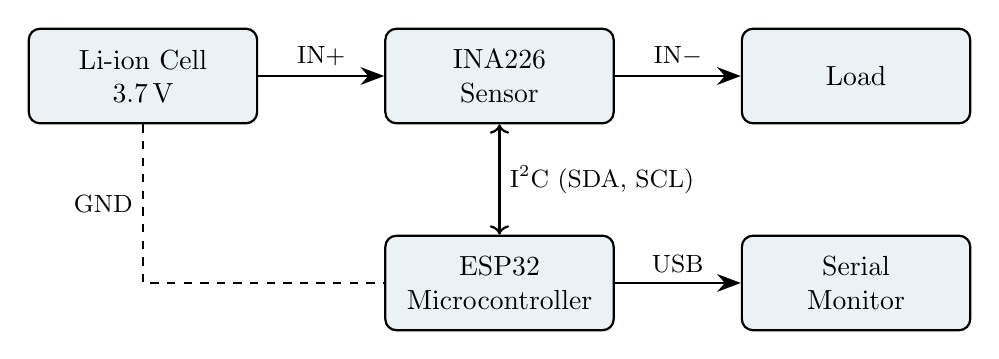
\begin{tikzpicture}[
  blk/.style={draw, rounded corners, thick, minimum width=2.9cm, minimum height=1.2cm, align=center, fill=accent!8},
  arr/.style={-{Stealth[length=3mm]}, thick},
  node distance=1.4cm and 1.6cm]
  \node[blk] (bat) {Li-ion Cell\\3.7\,V};
  \node[blk, right=of bat] (ina) {INA226\\Sensor};
  \node[blk, right=of ina] (load) {Load};
  \node[blk, below=of ina] (esp) {ESP32\\Microcontroller};
  \node[blk, right=of esp] (mon) {Serial\\Monitor};
  \draw[arr] (bat) -- node[above]{\small IN+} (ina);
  \draw[arr] (ina) -- node[above]{\small IN$-$} (load);
  \draw[arr, <->] (ina) -- node[right]{\small I\textsuperscript{2}C (SDA, SCL)} (esp);
  \draw[arr] (esp) -- node[above]{\small USB} (mon);
  \draw[thick, dashed] (bat.south) |- node[pos=0.25, left]{\small GND} (esp.west);
\end{tikzpicture}
\caption{Block diagram of the Battery Management System}
\label{fig:block}
\end{figure}

\section{Circuit Connections}
\begin{table}[H]
\centering
\caption{Circuit connections}
\label{tab:conn}
\begin{tabularx}{\linewidth}{llX}
\toprule
\textbf{From} & \textbf{To} & \textbf{Purpose} \\
\midrule
Battery + & INA226 IN+ & Battery voltage into the sensor \\
INA226 IN$-$ & Load + & All current passes through the shunt \\
Load $-$ & Battery $-$ & Completes the circuit \\
INA226 SDA & ESP32 GPIO 21 & I\textsuperscript{2}C data \\
INA226 SCL & ESP32 GPIO 22 & I\textsuperscript{2}C clock \\
INA226 VCC & ESP32 3.3\,V & Sensor supply \\
INA226 GND & Battery $-$ and ESP32 GND & Common ground reference \\
\bottomrule
\end{tabularx}
\end{table}

A common ground between the battery, the sensor and the ESP32 is essential, because all voltage measurements are made with respect to ground.

\section{Component Selection}
\begin{table}[H]
\centering
\caption{Components and justification}
\label{tab:comp}
\begin{tabularx}{\linewidth}{lX}
\toprule
\textbf{Component} & \textbf{Reason for selection} \\
\midrule
ESP32 & Low cost, fast (up to 240\,MHz), built-in I\textsuperscript{2}C, plenty of memory, and built-in Wi-Fi/Bluetooth for future remote monitoring. \\
INA226 & Measures both bus voltage and shunt current in one chip with 16-bit resolution; communicates over two I\textsuperscript{2}C wires; supports bidirectional current (charging and discharging). \\
0.1\,$\Omega$ shunt & Standard value on INA226 modules; gives a full-scale range of about 0.8\,A with very small power loss. \\
3.7\,V Li-ion cell & The most common rechargeable cell in portable electronics. \\
Serial Monitor & Simple display that requires no extra hardware. \\
Potentiometer (simulation) & Acts as an adjustable load/charger to test both current directions. \\
\bottomrule
\end{tabularx}
\end{table}

% =====================================================================
\chapter{Working Principle and Algorithm}\label{ch:principle}

\section{Overview}
The system works like a fuel meter for a battery. All current going into or out of the battery passes through the 0.1\,$\Omega$ shunt resistor of the INA226. The INA226 measures the tiny voltage across it to find the current, and it also measures the battery voltage. The ESP32 reads these values over I\textsuperscript{2}C and estimates the SoC in two steps.

\section{Step 1: Initial SoC from Voltage}
At start-up, the battery voltage is measured and compared with the lookup table (Table~\ref{tab:ocv}). If the voltage lies between two table points $(V_{i-1}, S_{i-1})$ and $(V_i, S_i)$, linear interpolation is used:
\begin{equation}
  \text{SoC} = S_{i-1} + (V - V_{i-1}) \cdot \frac{S_i - S_{i-1}}{V_i - V_{i-1}}
\end{equation}

\textbf{Example:} for $V = 3.96$\,V, the neighbouring points are 3.92\,V (70\,\%) and 4.00\,V (80\,\%):
\[
\text{SoC} = 70 + (3.96 - 3.92)\cdot\frac{80-70}{4.00-3.92} = 70 + 0.04 \times 125 = 75\,\%
\]
This percentage is converted to charge: for a 100\,mAh cell, $Q_0 = 100 \times 0.75 = 75$\,mAh.

The battery should be at rest at this moment; otherwise the voltage sag under load gives a lower starting value.

\section{Step 2: Coulomb Counting}
Every second, the current $I$ (mA) and the elapsed time $\Delta t$ (hours) are used to update the remaining charge according to Equation~\eqref{eq:cc}. Since \texttt{millis()} returns milliseconds:
\begin{equation}
  \Delta t\,(\text{h}) = \frac{\Delta t\,(\text{ms})}{3\,600\,000}
\end{equation}

\textbf{Example:} discharging at 400\,mA for 1\,s:
\[
\Delta Q = 400 \times \frac{1000}{3\,600\,000} = 0.111\ \text{mAh}
\]
Because discharging current is positive and charging current is negative, the same equation automatically decreases the charge while discharging and increases it while charging. The result is limited to the range $0 \le Q \le Q_{\text{capacity}}$, and the SoC is then calculated with Equation~\eqref{eq:soc}.

\section{True Battery Voltage}
The INA226 measures the \emph{bus voltage} on the load side of the shunt. The true battery voltage is therefore:
\begin{equation}
  V_{\text{battery}} = V_{\text{bus}} + V_{\text{shunt}}
\end{equation}

\section{Mode and Status Logic}
\begin{table}[H]
\centering
\caption{System response to different operating conditions}
\label{tab:modes}
\begin{tabularx}{\linewidth}{lX}
\toprule
\textbf{Condition} & \textbf{Response} \\
\midrule
$I > +20$\,mA & Mode DISCHARGING; SoC decreases; voltage drops slightly \\
$I < -20$\,mA & Mode CHARGING; SoC increases \\
$|I| \le 20$\,mA & Mode IDLE; SoC constant (dead zone avoids flicker from noise) \\
SoC $\le 20$\,\% & Status LOW (charge battery) \\
SoC $\ge 95$\,\% & Status FULL \\
Otherwise & Status OK \\
Sensor not found & Error message; program stops safely \\
\bottomrule
\end{tabularx}
\end{table}

\section{Flowchart}
\begin{figure}[H]
\centering
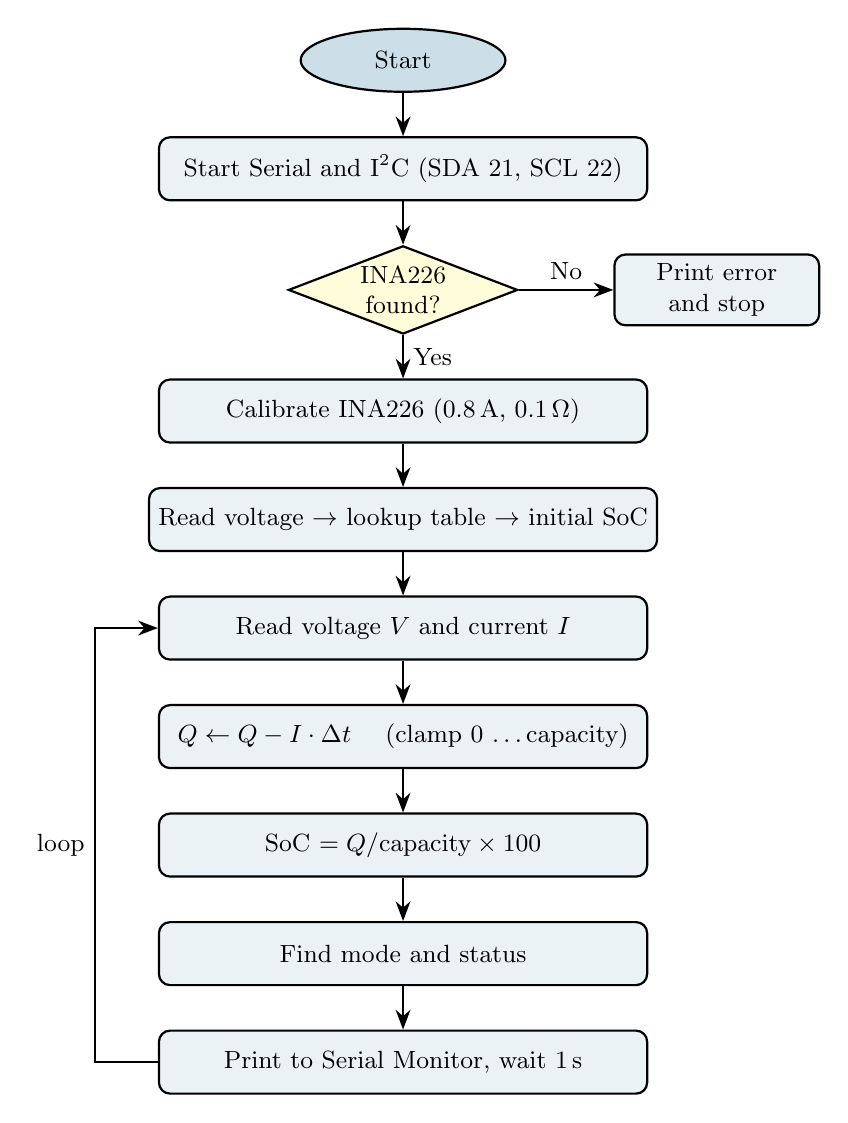
\begin{tikzpicture}[
  node distance=0.55cm,
  proc/.style={draw, thick, rectangle, rounded corners, minimum width=6.2cm, minimum height=0.8cm, align=center, fill=accent!8, font=\small},
  term/.style={draw, thick, ellipse, minimum width=2.6cm, minimum height=0.8cm, fill=accent!20, font=\small},
  dec/.style={draw, thick, diamond, aspect=2.6, align=center, fill=yellow!15, font=\small, inner sep=1pt},
  arr/.style={-{Stealth[length=2.5mm]}, thick}]
  \node[term] (start) {Start};
  \node[proc, below=of start] (init) {Start Serial and I\textsuperscript{2}C (SDA 21, SCL 22)};
  \node[dec, below=of init] (found) {INA226\\found?};
  \node[proc, right=1.2cm of found, minimum width=2.6cm] (err) {Print error\\and stop};
  \node[proc, below=of found] (cal) {Calibrate INA226 (0.8\,A, 0.1\,$\Omega$)};
  \node[proc, below=of cal] (v0) {Read voltage $\rightarrow$ lookup table $\rightarrow$ initial SoC};
  \node[proc, below=of v0] (read) {Read voltage $V$ and current $I$};
  \node[proc, below=of read] (cc) {$Q \leftarrow Q - I \cdot \Delta t$ \quad (clamp 0 \ldots capacity)};
  \node[proc, below=of cc] (soc) {SoC $= Q / \text{capacity} \times 100$};
  \node[proc, below=of soc] (mode) {Find mode and status};
  \node[proc, below=of mode] (print) {Print to Serial Monitor, wait 1\,s};
  \draw[arr] (start) -- (init);
  \draw[arr] (init) -- (found);
  \draw[arr] (found) -- node[above]{\small No} (err);
  \draw[arr] (found) -- node[right]{\small Yes} (cal);
  \draw[arr] (cal) -- (v0);
  \draw[arr] (v0) -- (read);
  \draw[arr] (read) -- (cc);
  \draw[arr] (cc) -- (soc);
  \draw[arr] (soc) -- (mode);
  \draw[arr] (mode) -- (print);
  \draw[arr] (print.west) -- ++(-0.8,0) |- node[pos=0.25, left]{\small loop} (read.west);
\end{tikzpicture}
\caption{Flowchart of the firmware}
\label{fig:flow}
\end{figure}

% =====================================================================
\chapter{Firmware Implementation}\label{ch:impl}

\section{Development Environment}
The firmware is written in Arduino C++ for the ESP32 (board: \emph{ESP32 Dev Module}) and uses the \texttt{INA226} library by Rob Tillaart for I\textsuperscript{2}C communication with the sensor. Output is sent to the Serial Monitor at 115200 baud.

\section{Program Modules}
\begin{itemize}
  \item \textbf{Settings:} battery capacity, shunt resistance, maximum current and the Li-ion lookup table.
  \item \textbf{\texttt{socFromVoltage()}:} converts a voltage into an SoC percentage using linear interpolation.
  \item \textbf{\texttt{setup()}:} starts Serial and I\textsuperscript{2}C, checks the INA226, calibrates it and sets the initial charge.
  \item \textbf{\texttt{loop()}:} every second reads the sensor, performs coulomb counting, calculates SoC, mode and status, and prints the results.
\end{itemize}

\section{Key Code Sections}

\subsection{Settings and Lookup Table}
\begin{lstlisting}
const float BATTERY_MAH = 2000.0;   // capacity of the cell (mAh)
const float SHUNT_OHM   = 0.1;      // shunt resistor on INA226 board
const float MAX_AMPS    = 0.8;      // max current for a 0.1 ohm shunt

const float volts[] = {3.00, 3.30, 3.60, 3.67, 3.71, 3.75, 3.79, 3.85, 3.92, 4.00, 4.10, 4.20};
const float socs[]  = {   0,    5,   10,   20,   30,   40,   50,   60,   70,   80,   90,  100};
\end{lstlisting}

\subsection{Voltage to SoC (Interpolation)}
\begin{lstlisting}
float socFromVoltage(float v) {
  if (v <= volts[0])          return 0;
  if (v >= volts[POINTS - 1]) return 100;
  for (int i = 1; i < POINTS; i++) {
    if (v < volts[i]) {
      return socs[i - 1] + (v - volts[i - 1]) * (socs[i] - socs[i - 1]) / (volts[i] - volts[i - 1]);
    }
  }
  return 100;
}
\end{lstlisting}

\subsection{Initialisation}
\begin{lstlisting}
Wire.begin(21, 22);                                  // SDA = 21, SCL = 22
if (!ina.begin()) { Serial.println("INA226 not found."); while (true) delay(1000); }
ina.setMaxCurrentShunt(MAX_AMPS, SHUNT_OHM, false);  // calibration

float startVoltage = ina.getBusVoltage() + ina.getShuntVoltage();
float startSoc     = socFromVoltage(startVoltage);
remainingMah       = BATTERY_MAH * startSoc / 100.0;
\end{lstlisting}

\subsection{Coulomb Counting}
\begin{lstlisting}
float current = ina.getCurrent_mA();             // + discharging, - charging
float hours   = (now - lastTime) / 3600000.0;    // ms -> hours
remainingMah  = remainingMah - current * hours;  // charge used or added
if (remainingMah < 0)           remainingMah = 0;
if (remainingMah > BATTERY_MAH) remainingMah = BATTERY_MAH;
float soc = remainingMah / BATTERY_MAH * 100.0;
\end{lstlisting}

\section{Sensor Calibration}
The call \texttt{setMaxCurrentShunt(0.8, 0.1)} configures the INA226 for the shunt value. The library computes the current resolution and the calibration register value:
\begin{equation}
  \text{Current\_LSB} = \frac{I_{\max}}{2^{15}} = \frac{0.8}{32768} \approx 24.4\,\mu\text{A}, \qquad
  \text{CAL} = \frac{0.00512}{\text{Current\_LSB} \cdot R_{\text{shunt}}} \approx 2097
\end{equation}
The INA226 then converts the shunt voltage directly into a current value.

\section{Repository Structure}
\begin{lstlisting}[language={}, numbers=none, basicstyle=\ttfamily\scriptsize]
bms/
|-- hardware/bms_soc/bms_soc.ino   Real-world firmware (BATTERY_MAH = 2000)
|-- wokwi-simulation/
|   |-- sketch.ino                 Same firmware (BATTERY_MAH = 100)
|   |-- diagram.json               Circuit definition
|   |-- ina226.chip.c / .json      Simulated INA226 sensor
|   |-- li-ion.chip.c / .json      Simulated 3.7 V Li-ion cell
|   `-- libraries.txt              INA226 library
|-- docs/                          Report and block diagram
|-- images/                        Screenshots
`-- README.md
\end{lstlisting}
Repository: \texttt{\githuburl}

% =====================================================================
\chapter{Simulation in Wokwi}\label{ch:sim}

\section{Why Simulation}
The INA226 sensor was not physically available, so the system was developed in the Wokwi online simulator. Wokwi simulates the ESP32 and runs the real compiled firmware. Simulation also avoids the risk and cost of experimenting with a real Li-ion battery.

Project link: \url{\wokwiurl}

\section{Custom Chips}
Wokwi has no built-in INA226 or battery part, so both were created as \emph{custom chips} written in C using the Wokwi Chips API. The firmware does not know it is running in simulation: it talks to the simulated INA226 exactly as it would to the real device.

\begin{figure}[H]
\centering
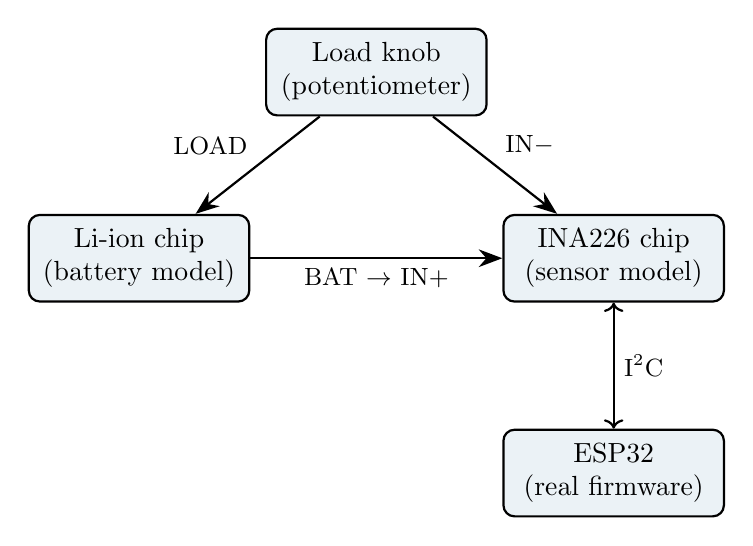
\begin{tikzpicture}[
  blk/.style={draw, rounded corners, thick, minimum width=2.8cm, minimum height=1.1cm, align=center, fill=accent!8},
  arr/.style={-{Stealth[length=3mm]}, thick}, node distance=1.6cm and 3.2cm]
  \node[blk] (bat) {Li-ion chip\\(battery model)};
  \node[blk, right=of bat] (ina) {INA226 chip\\(sensor model)};
  \node[blk, above=1.8cm of $(bat)!0.5!(ina)$] (pot) {Load knob\\(potentiometer)};
  \node[blk, below=of ina] (esp) {ESP32\\(real firmware)};
  \draw[arr] (bat) -- node[below]{\small BAT $\to$ IN+} (ina);
  \draw[arr] (pot) -- node[above left]{\small LOAD} (bat);
  \draw[arr] (pot) -- node[above right]{\small IN$-$} (ina);
  \draw[arr, <->] (ina) -- node[right]{\small I\textsuperscript{2}C} (esp);
\end{tikzpicture}
\caption{Structure of the Wokwi simulation}
\label{fig:simblock}
\end{figure}

\section{Load Knob}
A potentiometer acts as the load or charger. In Wokwi its output is 0--5\,V, which both chips convert to a current:
\begin{equation}
  I\ (\text{mA}) = \left( 2 \cdot \frac{V_{\text{knob}}}{5} - 1 \right) \times 800
\end{equation}
Turning the knob fully left gives $-800$\,mA (charging), the middle gives 0\,mA and fully right gives $+800$\,mA (discharging). A dead zone of $\pm$20\,mA around the middle is treated as zero.

\section{Li-ion Battery Model}
The battery chip runs every 100\,ms and:
\begin{enumerate}
  \item reads the knob to obtain the current;
  \item updates its own internal charge (this acts as the ``true'' value);
  \item converts the charge to a resting voltage using the same Li-ion curve (Table~\ref{tab:ocv});
  \item subtracts the voltage drop across an internal resistance of 0.1\,$\Omega$, so the voltage sags under load like a real cell;
  \item outputs this terminal voltage on its BAT pin;
  \item prints its actual charge to the Chips Console every 5\,s.
\end{enumerate}
\begin{equation}
  V_{\text{terminal}} = V_{\text{OCV}}(\text{SoC}) - I \cdot R_{\text{internal}}
\end{equation}
The simulated cell has a capacity of 100\,mAh so that changes are visible within minutes.

\section{INA226 Sensor Model}
The INA226 chip samples its IN+ (battery voltage) and IN$-$ (knob) pins every 10\,ms and converts the values into the same register format as the real device:
\begin{itemize}
  \item Shunt voltage register: $V_{\text{shunt}} / 2.5\,\mu$V
  \item Bus voltage register: $V_{\text{bus}} / 1.25$\,mV, where $V_{\text{bus}} = V_{\text{battery}} - I \cdot R_{\text{shunt}}$
  \item Current register: shunt register $\times$ CAL $/$ 2048 (as in the datasheet)
  \item Manufacturer ID \texttt{0x5449} (``TI'') and die ID \texttt{0x2260}
\end{itemize}
When the ESP32 writes a register number and reads two bytes over I\textsuperscript{2}C, the chip returns the value high byte first, exactly as the real INA226 does. This is why the same firmware works both in Wokwi and on real hardware.

\section{Simulation Circuit}
\screenshot{circuit.png}{Complete circuit in Wokwi: ESP32, INA226, Li-ion cell and load knob}{fig:circuit}

% =====================================================================
\chapter{Testing and Results}\label{ch:test}

\section{Test Procedure}
Each module was first checked on its own (sensor detection, voltage reading, current reading) and then the complete system was tested by turning the load knob to create discharging, charging and idle conditions. The SoC calculated by the ESP32 (Serial Monitor) was compared with the actual charge of the simulated battery (Chips Console).

\section{Test Cases}
\begin{table}[H]
\centering
\caption{Functional test cases}
\label{tab:tests}
\begin{tabularx}{\linewidth}{lXXc}
\toprule
\textbf{Test} & \textbf{Input} & \textbf{Observed output} & \textbf{Result} \\
\midrule
Sensor detection & Start simulation & INA226 detected, initial SoC printed & Pass \\
Discharge & Knob fully right & $+$799.9\,mA, DISCHARGING, SoC falling, voltage 3.905\,$\to$\,3.887\,V & Pass \\
Charge & Knob fully left & $-$799.9\,mA, CHARGING, SoC rising, voltage $\approx$4.05\,V & Pass \\
Idle & Knob at middle & $\approx$0\,mA, IDLE, SoC constant & Pass \\
Low status & Discharge below 20\,\% & Status LOW & Pass \\
Full status & Charge above 95\,\% & Status FULL & Pass \\
\bottomrule
\end{tabularx}
\end{table}

\section{Accuracy Verification}
At 800\,mA on a 100\,mAh cell, the expected change in 5 seconds is:
\[
\Delta Q = 800 \times \frac{5}{3600} = 1.11\ \text{mAh} = 1.11\,\%
\]
The Chips Console showed the actual battery charge falling from 78.9\,\% to 77.8\,\% to 76.7\,\% in 5-second steps, i.e.\ 1.1\,\% per step, and the SoC calculated by the ESP32 decreased at the same rate. This confirms that the coulomb counting is correct.

When the knob was not at the middle position at start-up, the initial voltage was read under load. The voltage sag then produced a starting SoC about 10\,\% lower than the true value, after which the two values changed in parallel. This confirms in practice why the initial estimate must be taken with the battery at rest.

\section{Sample Output}
\begin{lstlisting}[language={}, numbers=none, basicstyle=\ttfamily\scriptsize]
===== Basic BMS - SoC Monitor =====
Start voltage: 4.000 V  ->  Start SoC: 80.0 %

Voltage: 3.905 V | Current:  799.9 mA | DISCHARGING | SoC:  68.1 % | Left:  68.1 mAh | OK
Voltage: 3.902 V | Current:  799.9 mA | DISCHARGING | SoC:  67.9 % | Left:  67.9 mAh | OK
Voltage: 4.053 V | Current: -799.9 mA | CHARGING    | SoC:  66.7 % | Left:  66.7 mAh | OK
Voltage: 4.054 V | Current: -799.9 mA | CHARGING    | SoC:  67.0 % | Left:  67.0 mAh | OK
\end{lstlisting}

\screenshot{serial-discharging.png}{Serial Monitor while discharging (knob turned right)}{fig:dis}
\screenshot{serial-charging.png}{Serial Monitor while charging (knob turned left)}{fig:chg}
\screenshot{chips-console.png}{Chips Console showing the actual charge of the simulated battery}{fig:chips}

\section{Issues Encountered and Solutions}
\begin{table}[H]
\centering
\caption{Issues found during development}
\label{tab:issues}
\begin{tabularx}{\linewidth}{XX}
\toprule
\textbf{Issue} & \textbf{Solution} \\
\midrule
Wokwi has no INA226 or battery part & Wrote custom chips in C that behave like the real devices \\
Potentiometers start at position 0, giving a wrong initial SoC & Set default knob positions in \texttt{diagram.json} \\
Lookup table first written for a 3.3\,V LiFePO4 cell & Replaced with a 3.7\,V Li-ion table \\
Wokwi knob outputs 0--5\,V, not 0--3.3\,V, so the knob direction appeared reversed & Changed the scaling in both chips to 5\,V \\
INA226 chip read stale analog values inside I\textsuperscript{2}C callbacks & Sampled the pins in a 10\,ms timer and used the stored values \\
A 2000\,mAh battery changes too slowly to demonstrate & Used a 100\,mAh simulated cell \\
\bottomrule
\end{tabularx}
\end{table}

% =====================================================================
\chapter{Performance and Efficiency}\label{ch:perf}

\begin{itemize}
  \item \textbf{Communication:} I\textsuperscript{2}C needs only two wires and each reading is just a few bytes.
  \item \textbf{Processing speed:} each update involves a few multiplications and one table lookup, which the ESP32 completes in microseconds. A 1\,s interval is sufficient because battery charge changes slowly.
  \item \textbf{Memory:} only a few variables and two small constant arrays are used, with no dynamic memory allocation, so memory use is very low and stable.
  \item \textbf{Sensor accuracy:} the INA226 offers 16-bit resolution (1.25\,mV bus, 2.5\,$\mu$V shunt). The shunt voltage is added back to obtain the true battery voltage, and coulomb counting avoids errors due to voltage sag.
  \item \textbf{Reliability:} SoC is clamped to 0--100\,\%; the sensor is checked before operation; a $\pm$20\,mA dead zone prevents mode flicker from noise.
  \item \textbf{Power:} the INA226 draws well under 1\,mA. The ESP32 is the main consumer and can use deep sleep in a future version.
  \item \textbf{Cost:} only two main components are required, and developing in simulation avoided buying or risking a real battery.
\end{itemize}

% =====================================================================
\chapter{Conclusion and Future Work}\label{ch:concl}

\section{Results}
\begin{itemize}
  \item Battery voltage and current were read correctly from the INA226 over I\textsuperscript{2}C.
  \item The initial SoC was estimated from voltage, then tracked smoothly by coulomb counting.
  \item Charging, Discharging and Idle modes and LOW / OK / FULL status were detected correctly.
  \item The SoC calculated by the ESP32 changed at the same rate as the actual charge of the simulated battery.
\end{itemize}

\section{Conclusion}
A simple and low-cost Battery Management System can provide a reliable battery level using only an ESP32 and an INA226. Combining a voltage-based initial estimate with continuous coulomb counting performs much better than using voltage alone. Developing the system in Wokwi with custom simulated components saved cost and time, and the same firmware is ready to run on real hardware by changing only the battery capacity.

\section{Limitations}
\begin{itemize}
  \item Tested only in simulation, not yet with a physical battery.
  \item Coulomb counting can drift slowly over long periods due to small measurement errors.
  \item The initial estimate is accurate only if the battery is at rest at start-up.
  \item No temperature measurement and no protection cut-off.
  \item Single cell only; the Serial Monitor requires a connected computer.
\end{itemize}

\section{Future Work}
\begin{itemize}
  \item Build and test the system with real hardware.
  \item Add a MOSFET switch for over-charge, over-discharge and over-current protection.
  \item Add a temperature sensor (e.g.\ NTC thermistor).
  \item Re-correct the SoC from voltage after long rest periods to remove drift.
  \item Support multiple cells in series with balancing.
  \item Add an OLED display or a Wi-Fi dashboard using the ESP32's built-in Wi-Fi.
  \item Use ESP32 deep sleep between readings to reduce power consumption.
\end{itemize}

% =====================================================================
\begin{thebibliography}{9}
\addcontentsline{toc}{chapter}{References}
\bibitem{ina226} Texas Instruments, \emph{INA226 High-Side or Low-Side Measurement, Bi-Directional Current and Power Monitor with I\textsuperscript{2}C Compatible Interface}, Datasheet. \url{https://www.ti.com/product/INA226}
\bibitem{esp32} Espressif Systems, \emph{ESP32 Series Datasheet}. \url{https://www.espressif.com/en/products/socs/esp32}
\bibitem{lib} R.\ Tillaart, \emph{INA226 Arduino Library}. \url{https://github.com/RobTillaart/INA226}
\bibitem{wokwi} Wokwi, \emph{Custom Chips API Documentation}. \url{https://docs.wokwi.com/chips-api/getting-started}
\bibitem{plett} G.\ L.\ Plett, \emph{Battery Management Systems, Volume I: Battery Modeling}, Artech House, 2015.
\end{thebibliography}

% =====================================================================
\appendix
\chapter{Source Code}

\section{Firmware (\texttt{bms\_soc.ino})}
\lstinputlisting{../hardware/bms_soc/bms_soc.ino}

\section{Simulated Li-ion Cell (\texttt{li-ion.chip.c})}
\lstinputlisting[language=C]{../wokwi-simulation/li-ion.chip.c}

\section{Simulated INA226 (\texttt{ina226.chip.c})}
\lstinputlisting[language=C]{../wokwi-simulation/ina226.chip.c}

\section{Circuit Definition (\texttt{diagram.json})}
\lstinputlisting[language={}]{../wokwi-simulation/diagram.json}

\end{document}
